\documentclass[12pt,a4paper]{report}

% =========================
% Packages
% =========================
\usepackage{fontspec}
\setmainfont{Latin Modern Roman}
\usepackage[a4paper,margin=1in]{geometry}
\usepackage{setspace}
\usepackage{graphicx}
\usepackage{booktabs}
\usepackage{longtable}
\usepackage{array}
\usepackage{enumitem}
\usepackage{float}
\usepackage{tikz}
\usetikzlibrary{arrows.meta,positioning,shapes.geometric,fit,calc}
\usepackage{amsmath}
\usepackage{hyperref}
\usepackage{titlesec}

\onehalfspacing
\setlength{\parindent}{0.5in}
\setlength{\parskip}{0.2em}

\hypersetup{
    colorlinks=true,
    linkcolor=blue,
    urlcolor=blue,
    citecolor=blue,
    pdftitle={AI-powered Personalized Learning Path Platform},
    pdfauthor={Project Team}
}

\titleformat{\chapter}[display]
  {\bfseries\Huge}
  {CHAPTER \thechapter}
  {10pt}
  {\Huge}

% =========================
% Project information
% =========================
\newcommand{\projecttitle}{AI-powered Personalized Learning Path Platform for Competency Assessment Exam Preparation}
\newcommand{\projecttitlevi}{Hệ thống cá nhân hóa lộ trình học và luyện thi Đánh giá năng lực tích hợp AI}

\begin{document}

% =========================
% Cover
% =========================
\begin{titlepage}
\centering
\vspace*{1.2cm}

{\Large \textbf{CAPSTONE PROJECT REPORT}\par}
\vspace{1.2cm}

{\Huge \textbf{\projecttitle}\par}
\vspace{0.8cm}

{\Large \projecttitlevi\par}

\vfill

\begin{tabular}{ll}
\textbf{Project Type:} & AI-powered Personalized Learning Platform\\
\textbf{Main Platforms:} & Mobile Application and Web Application\\
\textbf{Core AI:} & Recommendation, Knowledge Tracing, Prediction, LLM, RAG\\
\textbf{Database:} & PostgreSQL\\
\textbf{Cloud:} & Microsoft Azure\\
\textbf{Version Control:} & GitHub
\end{tabular}

\vfill

{\large \textbf{Project Team}\par}
\vspace{0.3cm}
\begin{tabular}{cl}
\textbf{Nguyễn Thúy Nhi } & Main Content\\
\textbf{Phan Đình Quân } & Research and Supplementation\\
\textbf{Nguyễn Phạm Quỳnh Như} & Diagrams and Models\\
\textbf{Trương Nguyễn Trí Cường } & Technical Review\\
\textbf{Nguyễn Trung Nguyên } & Integration and LaTeX Formatting

\end{tabular}

\vfill
{\large Academic Year 2026\par}
\end{titlepage}

\hypersetup{pageanchor=false}
\pagenumbering{roman}

% =========================
% Abstract
% =========================
\chapter*{Abstract}
\addcontentsline{toc}{chapter}{Abstract}

Competency Assessment Examinations have become an important admission pathway in Vietnam. Unlike traditional examinations that primarily emphasize memorized knowledge, competency assessment focuses on logical reasoning, analytical thinking, reading comprehension, quantitative reasoning, and problem solving.

This project proposes an AI-powered personalized learning platform that continuously analyzes students' academic performance, assessment results, and learning behavior to generate and update individualized learning paths. The platform supports diagnostic assessment, adaptive practice, personalized study planning, AI-assisted tutoring, learning analytics, and examination performance prediction.

The proposed ecosystem consists of a student mobile application, a web portal for teachers and academic administrators, a parent monitoring portal, backend services, AI services, and analytics components. The planned technology stack includes Flutter, ReactJS/Next.js, ASP.NET Core Web API or Node.js, PostgreSQL, JWT/OAuth2, large language models, Retrieval-Augmented Generation (RAG), recommendation systems, knowledge tracing, machine learning, Qdrant or Pinecone, Microsoft Azure, and GitHub Actions.

\textbf{Keywords:} personalized learning, competency assessment, adaptive learning, AI Tutor, RAG, learning analytics, recommendation system, knowledge tracing.

\tableofcontents
\listoffigures
\listoftables

\clearpage
\pagenumbering{arabic}
\hypersetup{pageanchor=true}

% ============================================================
% CHAPTER 1
% ============================================================
\chapter{INTRODUCTION}

\section{Background}

In recent years, Competency Assessment Examinations have become one of the primary admission methods adopted by many universities in Vietnam. These examinations emphasize logical reasoning, analytical thinking, reading comprehension, quantitative reasoning, and problem-solving abilities.

Many existing online learning platforms provide identical learning content and predefined study plans for every learner. Such a static approach does not sufficiently consider individual differences in academic background, learning pace, target scores, available study time, or knowledge mastery.

As a result, students may spend excessive time reviewing topics they have already mastered while weaker areas receive insufficient practice. Teachers and parents may also lack effective tools for monitoring learning progress and competency development.

\section{Problem Statement}

The main problem addressed by this project is the lack of an adaptive learning environment that can continuously analyze learner performance and adjust study activities according to individual needs.

The proposed platform addresses this problem by maintaining a learner profile, generating personalized learning paths, recommending adaptive practice, providing AI-assisted tutoring, and visualizing learning analytics.

\section{Project Objectives}

The project aims to:

\begin{enumerate}
    \item Conduct diagnostic assessments to identify strengths and weaknesses.
    \item Generate personalized learning paths based on competency, target score, and preparation time.
    \item Recommend adaptive lessons and practice questions.
    \item Provide an AI Tutor for explanations, concept clarification, summarization, and additional questions.
    \item Monitor learning progress through analytics dashboards.
    \item Predict examination performance and identify potential risks.
    \item Provide teachers and parents with tools for monitoring learner progress.
\end{enumerate}

\section{Scope}

The proposed scope includes four major user groups: Administrator, Teacher/Academic Manager, Student, and Parent. The platform also contains AI services that analyze learning profiles, predict performance, explain questions, and generate additional practice.

\section{Project Deliverables}

The expected products are:

\begin{itemize}
    \item Student mobile application.
    \item Web portal for teachers and academic administrators.
    \item Parent portal.
    \item Backend platform for learning data management.
    \item AI Recommendation Engine.
    \item AI Tutor integrated with LLM and RAG.
    \item Learning Analytics Dashboard.
    \item Examination Performance Prediction Module.
    \item Personalized Learning Path Management Module.
\end{itemize}

% ============================================================
% CHAPTER 2
% ============================================================
\chapter{REQUIREMENT ANALYSIS}

\section{Stakeholders and System Roles}

\begin{longtable}{p{0.22\textwidth}p{0.68\textwidth}}
\toprule
\textbf{Role} & \textbf{Main Responsibilities}\\
\midrule
Administrator & Manage users, roles, courses, competency frameworks, question banks, learning resources, AI services, and system settings.\\
Teacher / Academic Manager & Develop learning materials, manage knowledge domains and learning objectives, create mock examinations, evaluate question quality, review student progress, and monitor recommendation quality.\\
Student & Complete diagnostic assessments, set target scores, follow personalized paths, practice adaptive exercises, take mock examinations, view dashboards, interact with AI Tutor, and receive recommendations.\\
Parent & Monitor student progress, view competency reports, receive alerts, track target score achievement, and monitor study schedules.\\
AI Recommendation Engine / Chatbot & Analyze learning profiles, predict examination performance, explain questions, provide answer explanations, answer academic questions, and generate additional practice.\\
\bottomrule
\end{longtable}

\section{Functional Requirements}

\subsection{FR1 -- Competency Diagnosis}
The system shall provide diagnostic assessments across multiple knowledge domains and cognitive skills.

\subsection{FR2 -- Learning Profile Generation}
The system shall analyze assessment results and behavioral indicators to establish a Learning Profile containing competency levels, learning preferences, and improvement areas.

\subsection{FR3 -- Personalized Learning Path}
The system shall generate a study roadmap according to the learner's profile, target examination score, and available preparation period.

\subsection{FR4 -- Adaptive Recommendation}
The system shall continuously analyze lesson, quiz, and mock examination performance and recommend subsequent learning activities with suitable difficulty and knowledge coverage.

\subsection{FR5 -- AI-assisted Learning Support}
The AI Tutor shall explain incorrect answers, summarize concepts, generate practice questions, recommend study techniques, and answer academic questions using contextual learning resources.

\subsection{FR6 -- Learning Analytics}
The system shall collect study duration, quiz performance, competency improvement, consistency, and engagement metrics and display them through dashboards.

\subsection{FR7 -- Examination Performance Prediction}
The system shall use historical learning data, competency progression, and behavioral analytics to estimate examination performance and identify potential risks.

\section{Non-Functional Requirements}

\begin{longtable}{p{0.30\textwidth}p{0.58\textwidth}}
\toprule
\textbf{Requirement} & \textbf{Target}\\
\midrule
Response time & Average response time below 3 seconds for standard operations.\\
Scalability & At least 1,000 concurrent active users.\\
Security & JWT authentication and Role-Based Access Control (RBAC).\\
Architecture & Modular separation of Mobile, Web, Backend, AI Services, and Analytics.\\
Data protection & Secure learning-data storage with scheduled backup and recovery.\\
Deployment & Cloud-native deployment with high availability and horizontal scalability.\\
Integration & APIs designed for future LMS and examination-framework integration.\\
\bottomrule
\end{longtable}

\section{Core Business Flows}

\begin{enumerate}
    \item \textbf{Competency Diagnosis and Learning Profile Generation}
    \item \textbf{Personalized Learning Path Planning}
    \item \textbf{Adaptive Learning and Continuous Recommendation}
    \item \textbf{AI-assisted Learning Support}
    \item \textbf{Learning Analytics and Progress Monitoring}
    \item \textbf{Examination Performance Prediction}
\end{enumerate}

% ============================================================
% CHAPTER 3
% ============================================================
\chapter{SYSTEM ANALYSIS \& DESIGN}

\section{Proposed System Architecture}

The platform is designed as a modular ecosystem separating client applications, backend services, AI services, and analytics.

\begin{figure}[H]
\centering
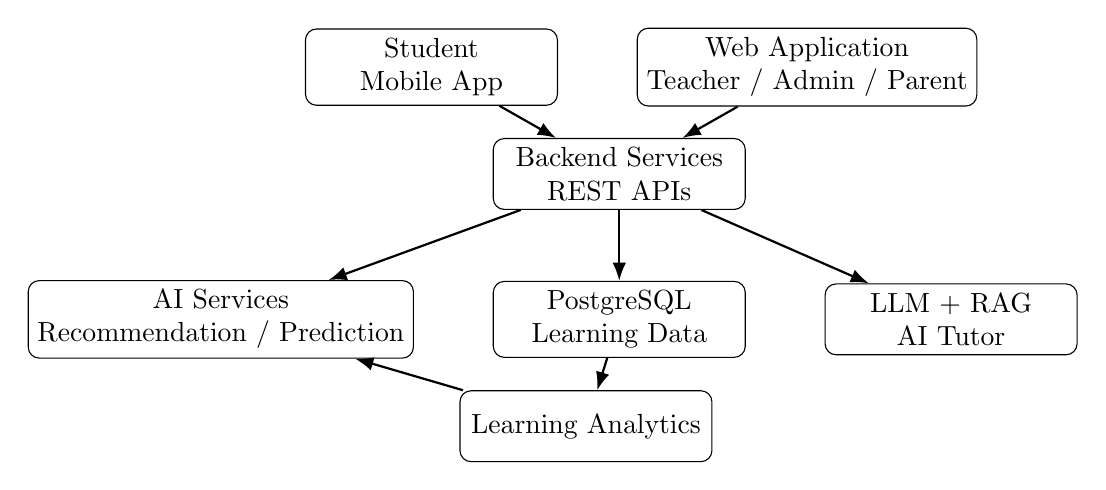
\begin{tikzpicture}[
    box/.style={rectangle, rounded corners, draw, minimum width=3.2cm, minimum height=0.9cm, align=center},
    arrow/.style={-{Latex}, thick},
    node distance=0.9cm and 1.0cm
]
\node[box] (mobile) {Student\\Mobile App};
\node[box, right=of mobile] (web) {Web Application\\Teacher / Admin / Parent};
\node[box, below=of $(mobile)!0.5!(web)$] (backend) {Backend Services\\REST APIs};
\node[box, below=of backend] (db) {PostgreSQL\\Learning Data};
\node[box, left=of db] (ai) {AI Services\\Recommendation / Prediction};
\node[box, right=of db] (rag) {LLM + RAG\\AI Tutor};
\node[box, below=of $(ai)!0.5!(rag)$] (analytics) {Learning Analytics};

\draw[arrow] (mobile) -- (backend);
\draw[arrow] (web) -- (backend);
\draw[arrow] (backend) -- (db);
\draw[arrow] (backend) -- (ai);
\draw[arrow] (backend) -- (rag);
\draw[arrow] (db) -- (analytics);
\draw[arrow] (analytics) -- (ai);
\end{tikzpicture}
\caption{High-level proposed system architecture}
\end{figure}

\section{Main Modules}

\begin{itemize}
    \item User and role management.
    \item Course and competency framework management.
    \item Learning material and question-bank management.
    \item Diagnostic assessment.
    \item Personalized learning path management.
    \item Adaptive recommendation.
    \item AI Tutor and RAG.
    \item Learning analytics.
    \item Examination performance prediction.
\end{itemize}

\section{Technology Stack}

\begin{longtable}{p{0.28\textwidth}p{0.60\textwidth}}
\toprule
\textbf{Component} & \textbf{Proposed Technology}\\
\midrule
Mobile & Flutter (Android and iOS)\\
Web & ReactJS / Next.js\\
Backend & ASP.NET Core Web API or Node.js (Express)\\
Database & PostgreSQL\\
Authentication & JWT and OAuth2\\
AI & LLMs, recommendation systems, knowledge tracing, machine learning\\
RAG & LangChain or Semantic Kernel\\
Vector database & Qdrant or Pinecone\\
Cloud & Microsoft Azure\\
CI/CD & GitHub Actions\\
Version control & GitHub\\
\bottomrule
\end{longtable}

\section{Data Flow Overview}

The overall learning data flow starts with assessment and learning activities. The backend stores the data, analytics services derive learning indicators, and AI components use these indicators to update recommendations and performance estimates.

% ============================================================
% CHAPTER 4
% ============================================================
\chapter{MOBILE APPLICATION}

\section{Purpose}

The mobile application is designed primarily for students and supports personalized learning, adaptive practice, AI Tutor interaction, and progress tracking.

\section{Main Student Features}

\begin{enumerate}
    \item Account authentication and profile management.
    \item Diagnostic assessment.
    \item Target score configuration.
    \item Personalized learning path.
    \item Daily study schedule.
    \item Lessons and learning materials.
    \item Adaptive quizzes and practice.
    \item Mock examinations.
    \item AI Tutor.
    \item Learning progress dashboard.
    \item Personalized recommendations.
    \item Predicted examination performance.
\end{enumerate}

\section{Personalized Learning Experience}

After completing the diagnostic assessment, the student receives a Learning Profile. The platform uses this profile together with the target score and available preparation period to construct a study roadmap.

During learning, the roadmap is updated according to quiz performance, competency progression, consistency, and engagement.

% ============================================================
% CHAPTER 5
% ============================================================
\chapter{WEB APPLICATION}

\section{Purpose}

The web application provides management and monitoring functions for administrators, teachers, academic managers, and parents.

\section{Administrator Functions}

Administrators manage:

\begin{itemize}
    \item Users and roles.
    \item Courses.
    \item Competency frameworks.
    \item Question banks.
    \item Learning resources.
    \item AI services and system settings.
    \item Overall platform operations.
\end{itemize}

\section{Teacher and Academic Manager Functions}

Teachers and academic managers can:

\begin{itemize}
    \item Develop and organize learning materials.
    \item Manage knowledge domains and learning objectives.
    \item Create and maintain mock examinations.
    \item Evaluate question quality.
    \item Review student learning progress.
    \item Monitor AI recommendation quality.
\end{itemize}

\section{Parent Monitoring}

The parent portal focuses on learning progress rather than content authoring. Parents can view competency development reports, target score achievement, learning alerts, schedules, and examination readiness.

% ============================================================
% CHAPTER 6
% ============================================================
\chapter{AI PERSONALIZATION}

\section{Personalization Concept}

The central idea of the platform is to replace a static curriculum with an adaptive learning journey. The system dynamically adjusts learning objectives, recommended lessons, exercises, and examination strategies according to the learner's competency and progress.

\section{Learning Profile}

A Learning Profile is generated from diagnostic assessment results and behavioral learning indicators. It represents:

\begin{itemize}
    \item Current competency levels.
    \item Areas of strength.
    \item Areas requiring improvement.
    \item Learning behavior indicators.
    \item Target examination score.
    \item Available preparation time.
\end{itemize}

\section{Recommendation Process}

A proposed recommendation cycle is:

\begin{enumerate}
    \item Collect assessment and learning activity data.
    \item Update competency estimates.
    \item Identify knowledge gaps.
    \item Prioritize learning objectives.
    \item Select suitable lessons and questions.
    \item Adjust difficulty and knowledge coverage.
    \item Monitor the next learning result.
    \item Repeat the cycle.
\end{enumerate}

\section{Knowledge Tracing}

Knowledge tracing is proposed as one of the models used to estimate changes in student competency over time. The report treats the specific model as an implementation choice to be finalized during development.

\section{Performance Prediction}

The AI engine is expected to use historical learning data, competency progression, and behavioral analytics to estimate examination performance and identify potential risks. The exact prediction model and evaluation metrics should be defined during implementation and testing.

% ============================================================
% CHAPTER 7
% ============================================================
\chapter{AI TUTOR \& RAG}

\section{AI Tutor Objectives}

The AI Tutor provides learning support throughout the student's learning journey. Its planned functions include:

\begin{itemize}
    \item Explaining incorrect answers.
    \item Clarifying difficult concepts.
    \item Summarizing knowledge.
    \item Generating additional practice questions.
    \item Recommending study techniques.
    \item Answering academic questions.
\end{itemize}

\section{Retrieval-Augmented Generation}

RAG is proposed to connect the language model with contextual learning resources. Instead of relying only on the model's general knowledge, the system can retrieve relevant learning content before generating a response.

\begin{figure}[H]
\centering
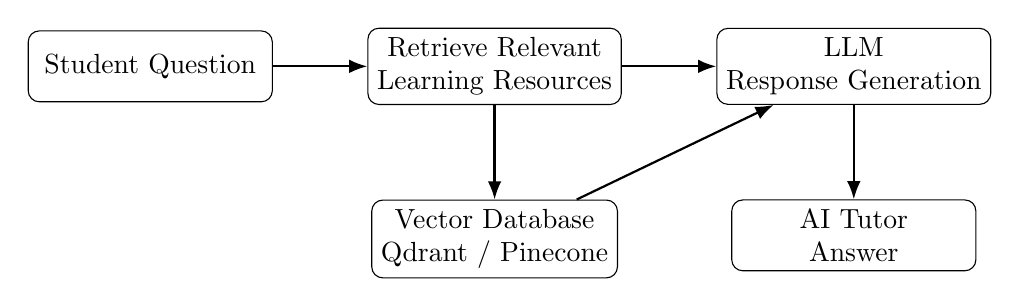
\begin{tikzpicture}[
    box/.style={rectangle, rounded corners, draw, minimum width=3.1cm, minimum height=0.9cm, align=center},
    arrow/.style={-{Latex}, thick},
    node distance=1.2cm
]
\node[box] (q) {Student Question};
\node[box, right=of q] (retrieve) {Retrieve Relevant\\Learning Resources};
\node[box, right=of retrieve] (llm) {LLM\\Response Generation};
\node[box, below=of retrieve] (vector) {Vector Database\\Qdrant / Pinecone};
\node[box, below=of llm] (answer) {AI Tutor\\Answer};

\draw[arrow] (q) -- (retrieve);
\draw[arrow] (retrieve) -- (llm);
\draw[arrow] (retrieve) -- (vector);
\draw[arrow] (vector) -- (llm);
\draw[arrow] (llm) -- (answer);
\end{tikzpicture}
\caption{Proposed AI Tutor and RAG flow}
\end{figure}

\section{RAG Technology}

The proposed implementation may use LangChain or Semantic Kernel for orchestration, an LLM service such as the OpenAI GPT API, and Qdrant or Pinecone as the vector database.

% ============================================================
% CHAPTER 8
% ============================================================
\chapter{LEARNING ANALYTICS}

\section{Purpose}

Learning analytics provides continuous monitoring of learning effectiveness, competency development, study habits, and engagement.

\section{Collected Indicators}

The proposed platform collects:

\begin{itemize}
    \item Study duration.
    \item Quiz performance.
    \item Competency improvement.
    \item Learning consistency.
    \item Engagement metrics.
    \item Mock examination results.
    \item Learning-path completion.
\end{itemize}

\section{Dashboards}

\subsection{Student Dashboard}

The student dashboard should help learners understand their progress, weak areas, recommended activities, study consistency, and examination readiness.

\subsection{Teacher Dashboard}

The teacher dashboard should provide progress monitoring, competency development information, and recommendation-quality monitoring.

\subsection{Parent Dashboard}

The parent dashboard should present competency development, target score achievement, alerts, study schedules, and examination readiness.

\section{Analytics and Personalization Loop}

Analytics is not only a reporting layer. It also provides input to the AI personalization engine. Learning data can therefore form a continuous feedback loop between student activity, analytics, competency estimation, and recommendation.

% ============================================================
% CHAPTER 9
% ============================================================
\chapter{IMPLEMENTATION}

\section{Implementation Architecture}

The implementation is planned around separated Mobile, Web, Backend, AI Services, and Analytics components. This modular structure supports future scaling and integration.

\section{Backend}

The backend may be implemented using ASP.NET Core Web API or Node.js (Express). It is responsible for APIs, authentication, learning data management, and communication with AI services.

\section{Database}

PostgreSQL is proposed as the primary database for structured learning data. The final database schema should cover users, roles, courses, competency frameworks, questions, assessments, learning activities, recommendations, and analytics data.

\section{Authentication and Authorization}

JWT and OAuth2 are proposed for authentication. Role-Based Access Control is used to separate permissions for administrators, teachers, students, and parents.

\section{AI Services}

AI-related services include:

\begin{itemize}
    \item Recommendation Engine.
    \item Knowledge Tracing.
    \item Student Performance Prediction.
    \item LLM-based AI Tutor.
    \item Retrieval-Augmented Generation.
\end{itemize}

\section{Cloud and CI/CD}

Microsoft Azure is proposed as the cloud deployment environment. GitHub Actions is proposed for CI/CD automation, while GitHub is used for version control.

\section{Implementation Status}

At the reporting stage, specific implementation details should be updated by the development team, including:

\begin{itemize}
    \item Actual backend framework selected.
    \item Final database schema.
    \item Implemented API endpoints.
    \item Actual AI models.
    \item Deployment architecture.
    \item CI/CD workflow.
    \item Screenshots of completed interfaces.
\end{itemize}

% ============================================================
% CHAPTER 10
% ============================================================
\chapter{TESTING \& EVALUATION}

\section{Testing Objectives}

Testing should verify functional correctness, technical requirements, AI behavior, performance, security, and usability.

\section{Functional Testing}

Functional tests should cover:

\begin{itemize}
    \item Authentication and authorization.
    \item Diagnostic assessment.
    \item Learning profile generation.
    \item Personalized learning path creation.
    \item Adaptive recommendations.
    \item AI Tutor interactions.
    \item Learning analytics.
    \item Examination performance prediction.
    \item Teacher and parent monitoring.
\end{itemize}

\section{Performance Testing}

The proposed non-functional requirement specifies an average response time below 3 seconds for standard operations and support for at least 1,000 concurrent active users.

Performance testing should therefore measure:

\begin{itemize}
    \item API response time.
    \item Concurrent-user capacity.
    \item Database performance.
    \item AI service latency.
    \item System behavior under load.
\end{itemize}

\section{AI Evaluation}

AI components require dedicated evaluation. Depending on the final implementation, evaluation may cover:

\begin{itemize}
    \item Recommendation relevance.
    \item Prediction performance.
    \item Knowledge-tracing consistency.
    \item AI Tutor answer quality.
    \item RAG retrieval relevance.
    \item Hallucination and unsupported-answer rate.
\end{itemize}

The final evaluation metrics should be selected according to the actual models and datasets used by the implementation team.

\section{Security Testing}

Security testing should include authentication, authorization, API access control, data protection, input validation, and backup/recovery procedures.

\section{Acceptance Criteria}

The system should be considered ready for final evaluation when the core business flows are implemented, major functional tests pass, performance requirements are measured, AI components are evaluated, and the required project deliverables are demonstrated.

% ============================================================
% CHAPTER 11
% ============================================================
\chapter{CONCLUSION \& FUTURE WORK}

\section{Conclusion}

This project proposes an AI-powered personalized learning platform for Competency Assessment Examination preparation. The system addresses the limitations of static learning plans by continuously analyzing student performance and behavior and using those signals to personalize learning activities.

The proposed platform combines mobile learning, web-based management, backend services, AI recommendation, knowledge tracing, performance prediction, AI-assisted tutoring, RAG, and learning analytics. The expected result is an adaptive learning ecosystem in which each learner follows an individualized study plan that evolves with academic performance and learning behavior.

\section{Future Work}

Future development may include:

\begin{itemize}
    \item More advanced competency and knowledge-tracing models.
    \item Improved recommendation algorithms.
    \item More examination frameworks and competency standards.
    \item Deeper LMS integration.
    \item More advanced learning analytics.
    \item Expanded AI Tutor capabilities.
    \item More robust RAG evaluation and knowledge-base management.
    \item Larger-scale cloud deployment and horizontal scaling.
    \item Additional predictive models for examination readiness.
\end{itemize}

\section{Expected Impact}

The platform is intended to provide students with individualized learning support while giving teachers and parents better visibility into learning progress. By combining adaptive learning, AI assistance, and analytics, the project aims to establish a scalable technical foundation for intelligent examination preparation.

% ============================================================
% TEAM CONTRIBUTION
% ============================================================
\chapter*{TEAM CONTRIBUTION}
\addcontentsline{toc}{chapter}{Team Contribution}

\begin{longtable}{p{0.18\textwidth}p{0.72\textwidth}}
\toprule
\textbf{Member} & \textbf{Responsibility}\\
\midrule
Person 1 & Main content: introduction, requirements, core system description, and report content ownership.\\
Person 2 & Research and supplementation: RBL topics, adaptive learning, intelligent tutoring, recommendation systems, knowledge tracing, learning analytics, and related technical background.\\
Person 3 & Diagrams and models: system architecture, business-flow diagrams, data-flow diagrams, AI/RAG flow, database and UML models.\\
Person 4 & Technical review: technology stack, architecture consistency, API/backend considerations, security, scalability, testing, and technical validation.\\
Person 5 & Integration and LaTeX formatting: merge chapters, standardize terminology, format figures/tables, manage references, compile the final report, and maintain the GitHub LaTeX project.\\
\bottomrule
\end{longtable}

\section*{Suggested Chapter Ownership}

A practical distribution for the 11 chapters is:

\begin{longtable}{p{0.25\textwidth}p{0.55\textwidth}}
\toprule
\textbf{Chapter} & \textbf{Primary Responsibility}\\
\midrule
Chapter 1 & Person 1\\
Chapter 2 & Person 1 + Person 2\\
Chapter 3 & Person 3 + Person 4\\
Chapter 4 & Person 1 + Person 4\\
Chapter 5 & Person 2 + Person 4\\
Chapter 6 & Person 2 + Person 3\\
Chapter 7 & Person 2 + Person 3\\
Chapter 8 & Person 2 + Person 4\\
Chapter 9 & Person 4\\
Chapter 10 & Person 4 + All members\\
Chapter 11 & Person 1 + All members\\
LaTeX integration & Person 5\\
Diagrams/models & Person 3\\
Final technical review & Person 4\\
Final compilation and formatting & Person 5\\
\bottomrule
\end{longtable}

\appendix

\chapter{REQUIREMENT TRACEABILITY SUMMARY}

\begin{longtable}{p{0.18\textwidth}p{0.30\textwidth}p{0.38\textwidth}}
\toprule
\textbf{ID} & \textbf{Requirement} & \textbf{Related Chapter}\\
\midrule
FR1 & Competency diagnosis & Chapters 2, 4, 6\\
FR2 & Learning profile generation & Chapters 2, 6\\
FR3 & Personalized learning path & Chapters 2, 4, 6\\
FR4 & Adaptive recommendation & Chapters 2, 4, 6\\
FR5 & AI-assisted learning support & Chapters 2, 7\\
FR6 & Learning analytics & Chapters 2, 8\\
FR7 & Performance prediction & Chapters 2, 6, 8\\
NFR1 & Response time below 3 seconds & Chapters 2, 9, 10\\
NFR2 & 1,000 concurrent users & Chapters 2, 9, 10\\
NFR3 & JWT and RBAC & Chapters 2, 5, 9, 10\\
NFR4 & Modular architecture & Chapters 3, 9\\
NFR5 & Secure storage and recovery & Chapters 3, 9, 10\\
NFR6 & Cloud scalability & Chapters 3, 9, 10\\
\bottomrule
\end{longtable}

\chapter{PROJECT TECHNOLOGY SUMMARY}

\begin{longtable}{p{0.30\textwidth}p{0.55\textwidth}}
\toprule
\textbf{Area} & \textbf{Technology / Approach}\\
\midrule
Mobile & Flutter\\
Web & ReactJS / Next.js\\
Backend & ASP.NET Core Web API or Node.js (Express)\\
Database & PostgreSQL\\
Authentication & JWT / OAuth2\\
LLM & OpenAI GPT API (proposed)\\
RAG & LangChain or Semantic Kernel (proposed)\\
Vector Database & Qdrant or Pinecone (proposed)\\
AI & Recommendation, Knowledge Tracing, Machine Learning, Prediction\\
Analytics & Educational Data Mining and Learning Analytics\\
Cloud & Microsoft Azure\\
CI/CD & GitHub Actions\\
Version Control & GitHub\\
\bottomrule
\end{longtable}

\end{document}
